\documentclass[12pt]{article}
\usepackage[utf8]{inputenc}
\usepackage{listings}
\usepackage[margin=1in]{geometry}
\usepackage{graphicx} % graficos
\usepackage{setspace}
\usepackage{xcolor}
\usepackage{color}
\usepackage{indentfirst}
\usepackage{listings}
\usepackage{isomath}
\usepackage{ulem}
\usepackage{caption}
\usepackage{algorithmicx}
\usepackage{algpseudocode}
\usepackage{algorithm}
% \algnewcommand{\LineComment}[1]{\State \(\triangleright\) #1}
\algnewcommand{\LineComment}[1]{\State \(\triangleright\) #1}
% \algrenewcomment[1]{\(\triangleright\) #1}
\graphicspath{ {/home/giovanni/famaf/2014/Modelos-y-Simulacion/trabajo_especial_I/informe/figuras/} }
\begin{document}


\begin{titlepage}
\begin{center}
\vspace*{1.5in}
\begin{Large}
\textbf{Modelos y Simulación}
\vspace{0.5in}

\textbf{Trabajo Especial I}

\vspace{0.3in}
\textbf{Modelo de Reparación}
% \begin{figure}[hbt]
% \noindent\makebox[\textwidth]{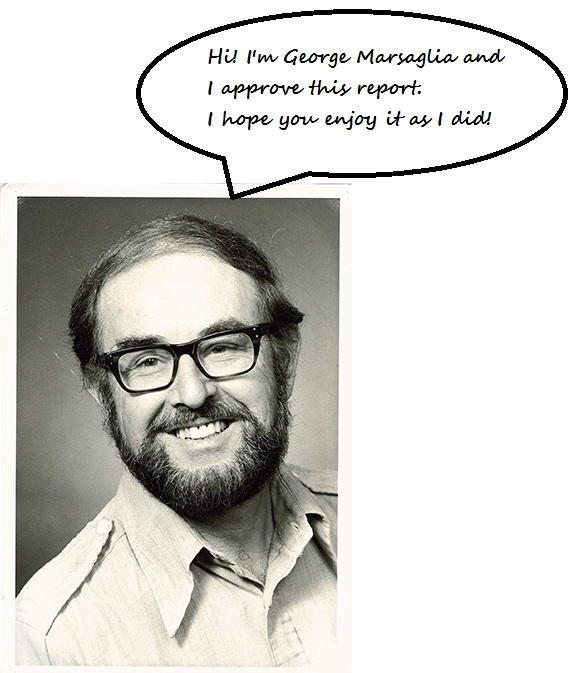
\includegraphics[scale=0.5]{gm}}
% \end{figure}

\vspace{1.5in}
Giovanni Rescia

\vspace*{0.4in}

FaMAF, UNC
\vspace*{.13in}

21 de Mayo de 2014
\end{Large}
\end{center}
\end{titlepage}

% \title{\textbf{Modelos y Simulación \\ \large Trabajo Especial I \\ \large Modelo de Reparación}}
\author{Giovanni Rescia \\ \\ \large FaMAF}
\date{21 de Mayo de 2014}



% \maketitle
\pagebreak
\section{Resumen}
\vspace{0.4in}
El objetivo de este trabajo es poder estimar mediante simulaciones,
la vida \'util de un lavadero con $N$ máquinas en funcionamiento,
$S$ máquinas de repuesto y $K$ operarios que reparan las máquinas
que se van rompiendo. La vida \'util estará representada por
"cuánto tiempo funciona el sistema hasta que hay menos de $N$
máquinas en funcionamiento" teniendo en cuenta las de repuesto
y aquellas que vayan reparando a lo largo del tiempo los operarios.
Y también poder responder a preguntas del tipo "para mejorar la media
del tiempo antes que el sistema falle, conviene agregar un operario
o una máquina?".

\pagebreak
\section{Introducción}
\vspace{0.4in}
Un lavadero de ropa automático, cuenta con $N$ máquinas lavadoras en servicio y con $S$ máquinas de
repuesto, todas ellas de idéntica marca, modelo y antigüedad. Además el lavadero cuenta con los servicios
de un técnico que repara las máquinas. Obviamente, el técnico repara las máquinas en serie, encargándose
de una sola por vez. El problema consiste en determinar el tiempo medio (y su correspondiente desviación
estándar) que transcurre hasta que el lavadero deja de ser operativo (fallo del sistema), esto es, el momento
en el que se tiene menos de $N$ máquinas en servicio, o lo que es lo mismo, posee mas de $S$ máquinas
defectuosas en el taller.

Todos los tiempos de funcionamiento de las maquinas hasta descomponerse son variables independientes
exponenciales con un tiempo medio hasta fallar de $T_{F}$ , y que el tiempo de reparación de una máquina
que ingresa a taller es una variable exponencial con tiempo medio igual a $T_{R}$ , independiente de todos los
anteriores.
\vspace{0.4in}
\subsection{Bases teóricas para la resolución del problema}
A continuación se presentan las bases teóricas en las cuales este modelo
está fuertemente basado para su resolución
\subsubsection{Cálculo de la Esperanza y la Varianza por la ley fuerte de los grandes números}
\vspace{0.2in}
{\bf Esperanza}
\vspace{0.15in}

{\bf Teorema:} Sea $X_1$,$X_2$,...,$X_n$ una sucesión de variables aleatorias independientes
e idénticamente distribuidas con media $\mu$, entonces vale que
\[\lim\limits_{n\rightarrow \infty}\frac{X_1+X_2+...+X_n}{n}=\mu\]

Basándonos en ese resultado, podemos obtener al correr el algoritmo $n$ veces para obtener la vida útil
del sistema y al dividirlo por $n$ obtendremos la esperanza (con $n$ suficientemente grande).
\vspace{0.3in}

{\bf Varianza}
\vspace{0.15in}

Para el cálculo de $\sigma^2$ utilizaremos el siguiente estimador insesgado (i.e, sea $\theta$ una v.a. entonces $\hat{\theta}$
es un estimador insesgado de $\theta$ si $E$[$\hat{\theta}$]=$\theta$).
Antes de dar un estimador insesgado de la varianza, daremos uno de la esperanza, ya que la varianza depende de la esperanza.
\pagebreak
% \vspace{0.3in}

{\bf Proposición:} Sea $X_1$,$X_2$,...,$X_n$ una sucesión de variables aleatorias independientes
e idénticamente distribuidas con media $\mu$, y sea
\[\bar{X}=\sum\limits_{i=1}^n \frac{X_i}{n}\]
entonces vale que
\[E[\bar{X}]=\mu\]

\vspace{0.2in}

\noindent Ahora que tenemos un estimador insesgado para $\mu$, tenemos la siguiente proposición:

\vspace{0.2in}

{\bf Proposición:} Sea $X_1$,$X_2$,...,$X_n$ una sucesión de variables aleatorias independientes
e idénticamente distribuidas con esperanza $\mu$ y varianza $\sigma^2$ y sea $\bar{X}$ un estimador insesgado de $\mu$ entonces si
\[S^2=\sum\limits_{i=1}^n \frac{(X_i - \bar{X})^2}{n-1}\]
entonces $S^2$ es un estimador insesgado para $\sigma^2$.
Por lo que la desviación estándar $\sigma$ es igual a $S$.
\vspace{0.2in}

\subsubsection{Generación de variables aleatorias uniformes continuas en el (0,1)}

Contamos con un método eficiente para generar una variable aleatoria $U\sim \mathcal{U}$(0,1).


Se podría considerar como la parte algorítmica más importante, ya que nos va a permitir
generar variables aleatorias exponenciales. (Se puede generar cualquier variable aleatoria
solo que en este problema solo nos interesan las exponenciales).
\vspace{0.2in}

\subsubsection{Tiempos de fallo y reparación de las máquinas}

Trabajamos bajo las siguientes hipótesis:
\begin{itemize}
 \item Todos los tiempos de funcionamiento de las máquinas hasta descomponerse son variables independientes
 exponenciales con un tiempo medio hasta fallar de 1 mes. Es decir, el tiempo de funcionamiento hasta
 descomponerse es una variable aleatoria $\sim\varepsilon$(1)
 \item El tiempo de reparación de una máquina que ingresa a taller es una variable exponencial con tiempo medio igual a 1/8 de mes,
 independiente de todos los anteriores. Es decir, el tiempo de reparación de una máquina es una variable aleatoria $\sim\varepsilon$(8)
\end{itemize}
\vspace{0.2in}
\pagebreak

\subsubsection{Generación de variables aleatorias exponenciales}

Gracias a que podemos generar una variable aleatoria $U\sim \mathcal{U}$(0,1)
podemos implementar un algoritmo para generar variables aleatorias $\sim\varepsilon(\lambda)$.

El pseudo código a continuación:

\vspace{0.14in}
\emph{Generar $X \sim\varepsilon(\lambda)$:}
  \begin{enumerate}
   \item Generar $U\sim \mathcal{U}$(0,1)
   \item $X\leftarrow -\frac{1}{\lambda}\log(U)$
  \end{enumerate}

Entonces los algoritmos para generar los tiempos de vida hasta que se descompone y hasta que se arregla una
máquina están dados por:
\vspace{0.14in}

\emph{Generar tiempo hasta descomponerse $X \sim\varepsilon(1)$:}
  \begin{enumerate}
   \item Generar $U\sim \mathcal{U}$(0,1)
   \item $X\leftarrow -log(U)$
  \end{enumerate}
\vspace{0.14in}

\emph{Generar tiempo hasta arreglo $X \sim\varepsilon(8)$:}
  \begin{enumerate}
   \item Generar $U\sim \mathcal{U}$(0,1)
   \item\indent$X\leftarrow -\frac{1}{8}\log(U)$
  \end{enumerate}
\pagebreak

\section{Pseudo Código para realizar la simulación}

(Nota: por cuestiones de espacio, el algoritmo fue separado en 3 partes:
la primera tiene las variables y sus respectivas inicializaciones, la segunda
parte describe el evento en que se rompe un máquina antes que otra sea arreglada, y
la tercer parte describe el evento en que se repara una máquina antes que otra falle)	 

\begin{algorithm}
\caption{Simuación con $n$ máquinas en funcionamiento, $s$ de repuesto y un operario}
\begin{algorithmic}[1]
\Procedure{Simulación}{}
\LineComment {Inicialización de variables}
\LineComment {Cantidad de máquinas en funcionamiento para que el sistema no falle}
\State $working\_machines \gets n$
\LineComment {Máquinas de repuesto}
\State $spare\_machines \gets s$
\State $system\_failure \gets False$
\LineComment {Tiempo final en meses (output)}
\State $T \gets 0$
\LineComment {Variable de tiempo}
\State $t \gets 0$
\LineComment {$broken\_machines$ va a marcar el estado del sistema; son
las máquinas rotas en el tiempo $t$. Esta variable va a cambiar cuando una
máquina falle o una máquina se repare}
\State $broken\_machines \gets 0$
\LineComment {Tiempo en que se reparó la última máquina}
\State $machine\_repair\_time \gets \infty$
\LineComment {Guardo los tiempos de falla de las máquinas en un conjunto,
por ende, está ordenado}
\State $machines\_failure\_time \gets \emptyset$
\LineComment {Generamos los tiempos de falla de las máquinas}
\For {$i \gets 1 \textrm{ \bf to } n$}
  \State $X \gets \varepsilon(1)$
  \State $machines\_failure\_time \gets machines\_failure\_time \cup \left\{ X \right\} $
\EndFor
    \algstore{myalg}
\end{algorithmic}
\end{algorithm}
\clearpage
\begin{algorithm}
  \ContinuedFloat
  \caption{Simuación con $n$ máquinas en funcionamiento, $s$ de repuesto y un operario(continuación)}
  \begin{algorithmic}
      \algrestore{myalg}
\LineComment {Mientras hallan menos máquinas rotas que de repuesto,
el sistema va a funcionar normalmente}
\While {$\textrm { \bf not } system\_failure$}
  \LineComment {Nos fijamos en la primer máquina en fallar}
  \State $t_1 \gets \textit{Menor elemento (tiempo) del conjunto}$
  \LineComment {Evento de tipo 1: falló una máquina antes que otra se arregle}
  \If {$t_1 < machine\_repair\_time$}
    \LineComment {Actualizamos el tiempo $t$}
    \State $t \gets t_1$
    \LineComment {Tenemos otra máquina rota, pues falló antes que se arrgle otra}
    \State $broken\_machines \gets broken\_machines + 1$
    \LineComment {Si hay más máquina en reparación que de repuesto, entonces
    el sistema falla, pues no me alcanza para tener $n$ en funcionamiento}
    \If {$broken\_machines > spare\_machines$}
      \LineComment {$T$ representa el tiempo total que el sistema estuvo en funcionamiento}
      \State $T \gets t$
      \LineComment {El sistema ha fallado}
      \State $system\_failure \gets True$
    \LineComment {Cuento con máquinas de repuesto, el sistema se mantiene estable}
    \Else
      \LineComment {Genero el tiempo que va a durar una de las máquinas de repuesto que pongo en funcionamiento}
      \State $X \gets \varepsilon(1)$
      \LineComment {Ya no necesito la primer máquina que falló, pues es reemplazada}
      \State $machines\_failure\_time \gets machines\_failure\_time - \left\{ t_1 \right\} $
      \LineComment {La máquina de repuesto va a entrar en funcionamiento en el momento $t$, y va durar
      $X$, por lo que la falla se producirá en el tiempo $X + t$}
      \State $machines\_failure\_time \gets machines\_failure\_time \cup \left\{ X + t \right\} $
    \EndIf
    \LineComment {Si hay una máquina esperando ser reparada, la reparo}
    \If {$broken\_machines == 1 $}
      \LineComment {Genero un tiempo de reparación de la máquina}
      \State $Y \gets \varepsilon(8)$
      \LineComment {La máquina se va a empezar a reparar en el tiempo $t$,
       y la reparación va a tomar un tiempo $Y$, por lo tanto, la reparación
       se va a completar en el tiempo $Y + t$}
      \State $machine\_repair\_time \gets Y + t$
      \EndIf
\algstore{myalg}
\end{algorithmic}
\end{algorithm}
\clearpage
\begin{algorithm}
\ContinuedFloat
\caption{Simuación con $n$ máquinas en funcionamiento, $s$ de repuesto y un operario(continuación)}
\begin{algorithmic}
\algrestore{myalg}
  \LineComment {Evento de tipo 2: una máquina es reparada antes que falle una que está en funcionamiento}
  \Else
    \LineComment {Actualizamos el tiempo $t$}
    \State $t \gets machine\_repair\_time$
    \LineComment {Reparé una máquina, por lo tanto tengo una máquina rota menos}
    \State $broken\_machines \gets broken\_machines - 1$
    \LineComment {Si todavía hay máquinas rotas, reparo una}
    \If {$broken\_machines > 0$}
      \LineComment {Genero un tiempo de reparación de la máquina}
      \State $Y \gets \varepsilon(8)$
      \LineComment {La máquina se va a empezar a reparar en el tiempo $t$,
       y la reparación va a tomar un tiempo $Y$, por lo tanto, la reparación
       se va a completar en el tiempo $Y + t$}
      \State $machine\_repair\_time \gets Y + t$
    \EndIf
    \LineComment {Si no hay máquinas rotas, entonces la próxima máquina va a tomar $\infty$ tiempo en ser
    reparada (pues no hay ninguna que reparar en este instante $t$)}
    \If {$broken\_machines == 0$}
      \LineComment {Restablezco el tiempo de reparación de la máquina}
      \State $machine\_repair\_time \gets \infty$
    \EndIf
  \EndIf
\EndWhile
\State {$\textbf{RETURN } T$}
\EndProcedure
\end{algorithmic}
\end{algorithm}

Este algoritmo describe una simulación para $n$ máquinas en funcionamiento, $s$ máquinas de repuesto
y un solo operario.
\clearpage

\subsection{Algoritmo para un sistema con dos operarios}

La lógica del algoritmo es casi la misma, hay que agregarle las siguientes líneas al algoritmo anterior
para poder lograr una simulación de un sistema con $n$ máquinas en funcionamiento, $s$ máquinas de repuesto
y dos operarios que arreglan máquinas. Las siguiente líneas de pseudo código se embeben justo después de la línea $53$
del algoritmo anterior (se van a mostrar las líneas $49$ a $53$ también para ponerlo en contexto).


\begin{algorithm}
\caption{Simuación con $n$ máquinas en funcionamiento, $s$ de repuesto y dos operarios}
\begin{algorithmic}
\Procedure{Simulación}{}
\If {$broken\_machines == 1 $}
  \LineComment {Genero un tiempo de reparación de la máquina}
  \State $Y \gets \varepsilon(8)$
  \LineComment {La máquina se va a empezar a reparar en el tiempo $t$,
  y la reparación va a tomar un tiempo $Y$, por lo tanto, la reparación
  se va a completar en el tiempo $Y + t$}
  \State $machine\_repair\_time \gets Y + t$
\EndIf
\LineComment {Si hay dos máquinas en reparación, es porque otra se rompió antes que la última
que entró en reparación se halla reparado. Como tengo otro operario más, la puedo poner a reparar}
\If {$broken\_machines == 2$}
  \LineComment {Genero un tiempo de reparación de la máquina}
  \State $Y \gets \varepsilon(8)$
  \LineComment {La máquina se va a empezar a reparar en el tiempo $t$,
  y la reparación va a tomar un tiempo $Y$, por lo tanto, la reparación
  se va a completar en el tiempo $Y + t$}
  \State $machine\_2\_repair\_time \gets Y + t$
  \LineComment {Como los eventos que observo son la reparación y el fallo de una máquina, 
  lo que me va a interesar obtener en este caso es la máquina que sea reparada en menor tiempo entre
  la máquina que estaba siendo reparada y la que acaba de entrar (en el tiempo $t$) a ser reparada}
  \State $machine\_repair\_time \gets \min \left\{ machine\_repair\_time, machine\_2\_repair\_time\right\}$
\EndIf
\EndProcedure
\end{algorithmic}
\end{algorithm}

\pagebreak

\section{Resultados obtenidos}
A continuación se muestran los resultados de la simulación. Para cada caso la Simuación
se corrió 100000 veces para calcular la Esperanza, tanto como la Varianza (por ende la desviación estándar)
y tanto como para obtener puntos para realizar los gráficos.


\subsection{Resultados con 5 máquinas en funcionamiento, 2 de repuesto y un operario}

% \noindent El siguiente gráfico podemos observar el estado del sistema actual:
\begin{figure}[hbt]
\noindent\makebox[\textwidth]{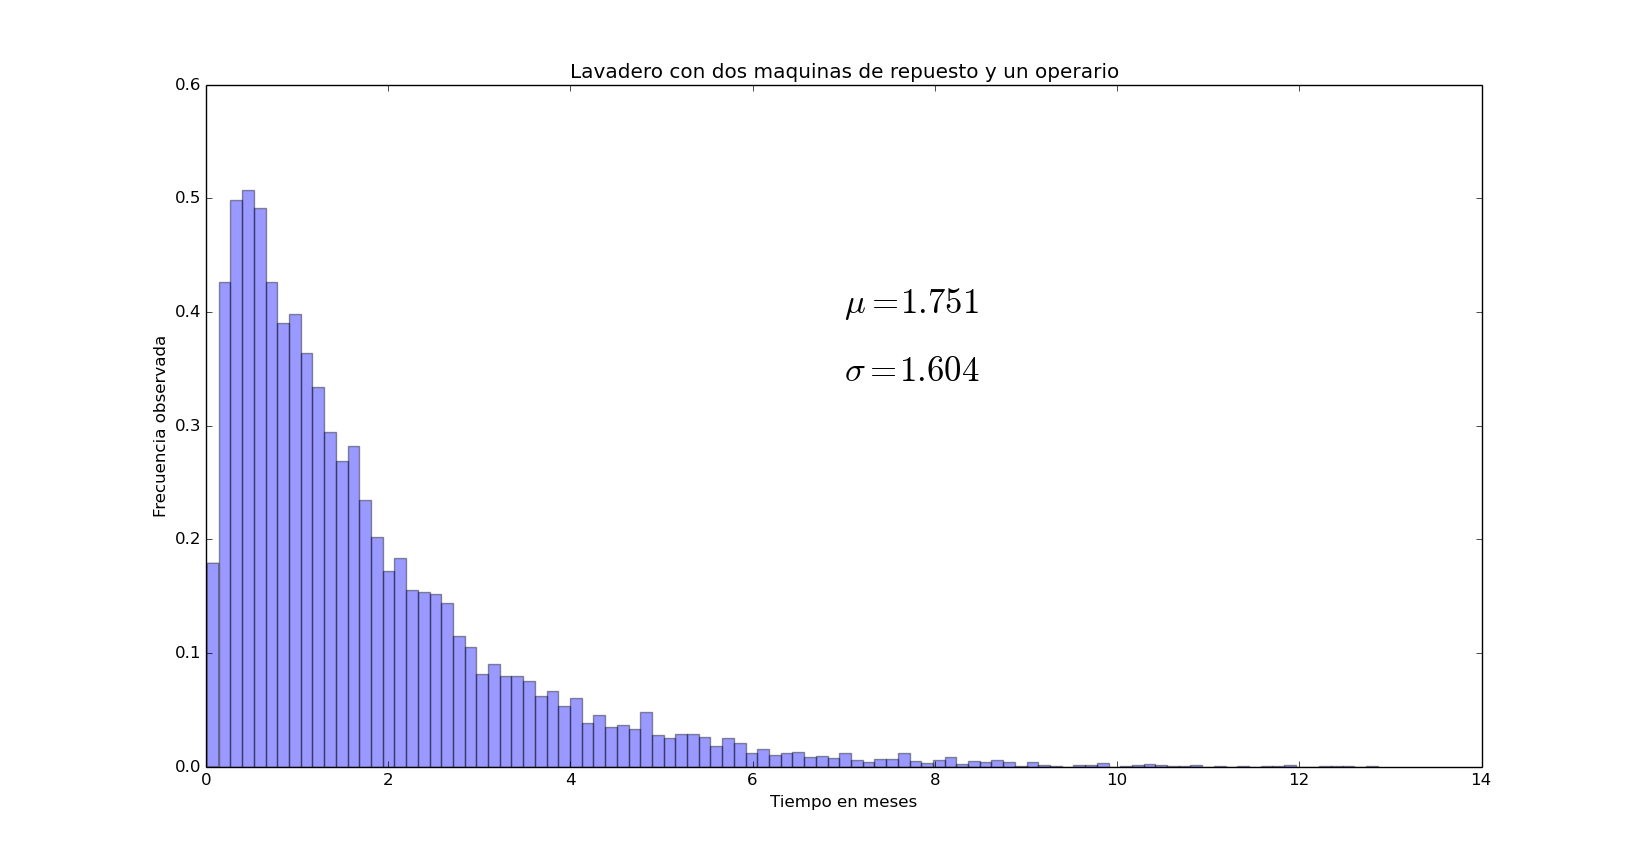
\includegraphics[scale=0.5]{figure_1}}
\end{figure}

Ahora, si uno quisiera mejorar el tiempo antes que el sistema falle (con 5 máquinas en funcionamiento),
podría elegir entre dos opciones: agregar un operario, o agregar una máquina de repuesto.

A continuación, resultados de la simulación para las dos posibles soluciones.

\pagebreak

\subsection{Solución 1: Agregar un operario}

\begin{figure}[hbt]
\noindent\makebox[\textwidth]{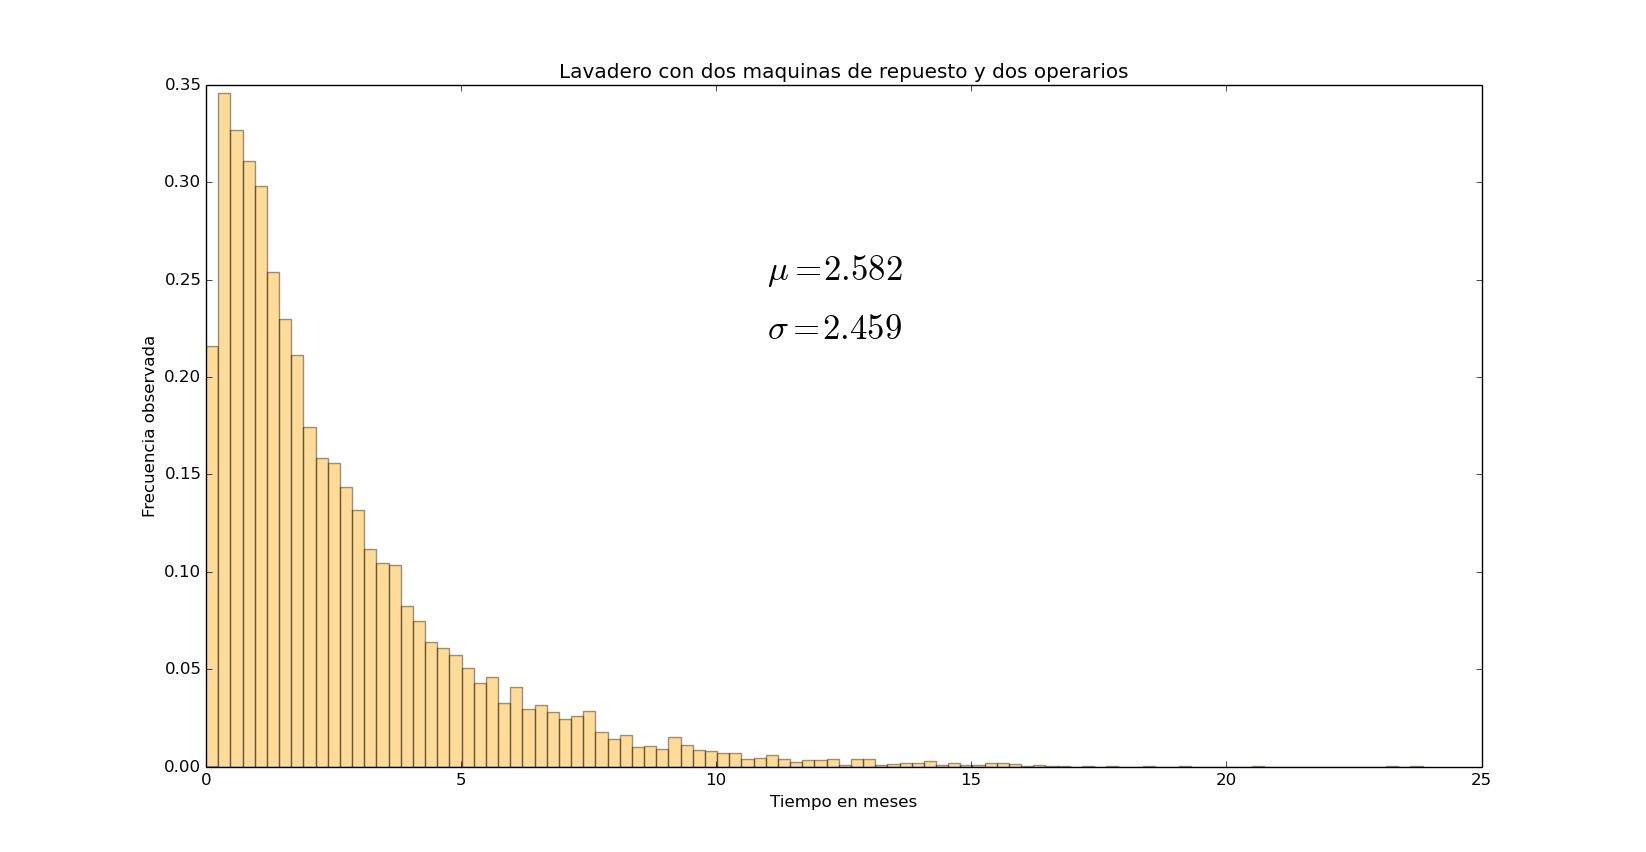
\includegraphics[scale=0.4]{figure_2}}
\end{figure}

Comparemos cómo ha cambiado el desempeño del sistema:

\begin{figure}[hbt]
\noindent\makebox[\textwidth]{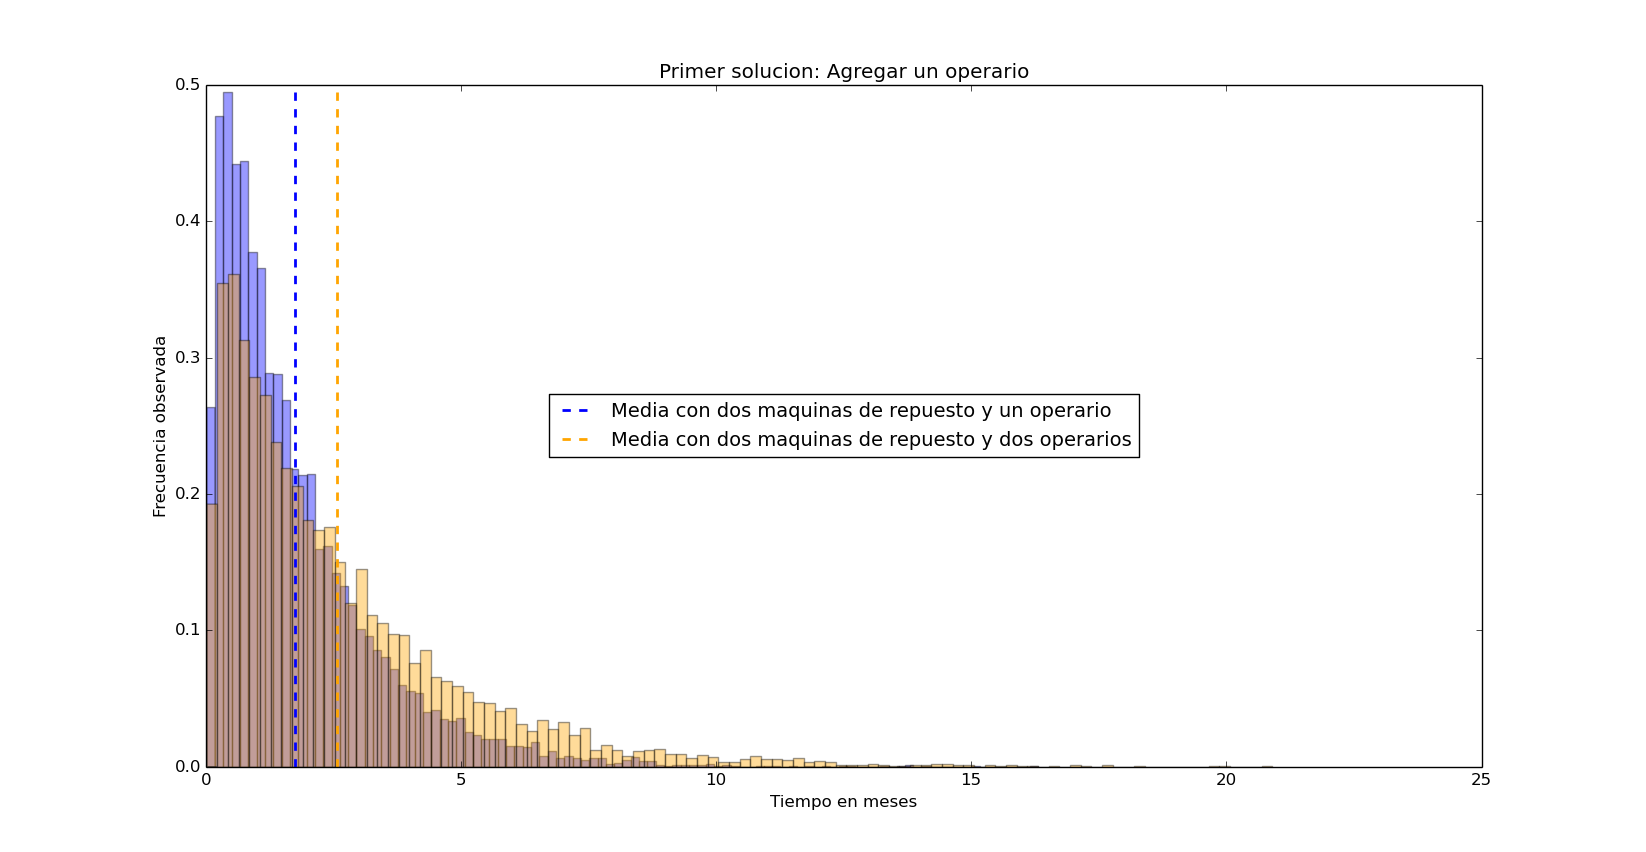
\includegraphics[scale=0.375]{figure_4}}
\end{figure}

Se puede observar una mejoría de aproximadamente 1 mes en el tiempo medio de falla del sistema.

\pagebreak

\subsection{Solución 2: Agregar una máquina de repuesto}

\begin{figure}[hbt]
\noindent\makebox[\textwidth]{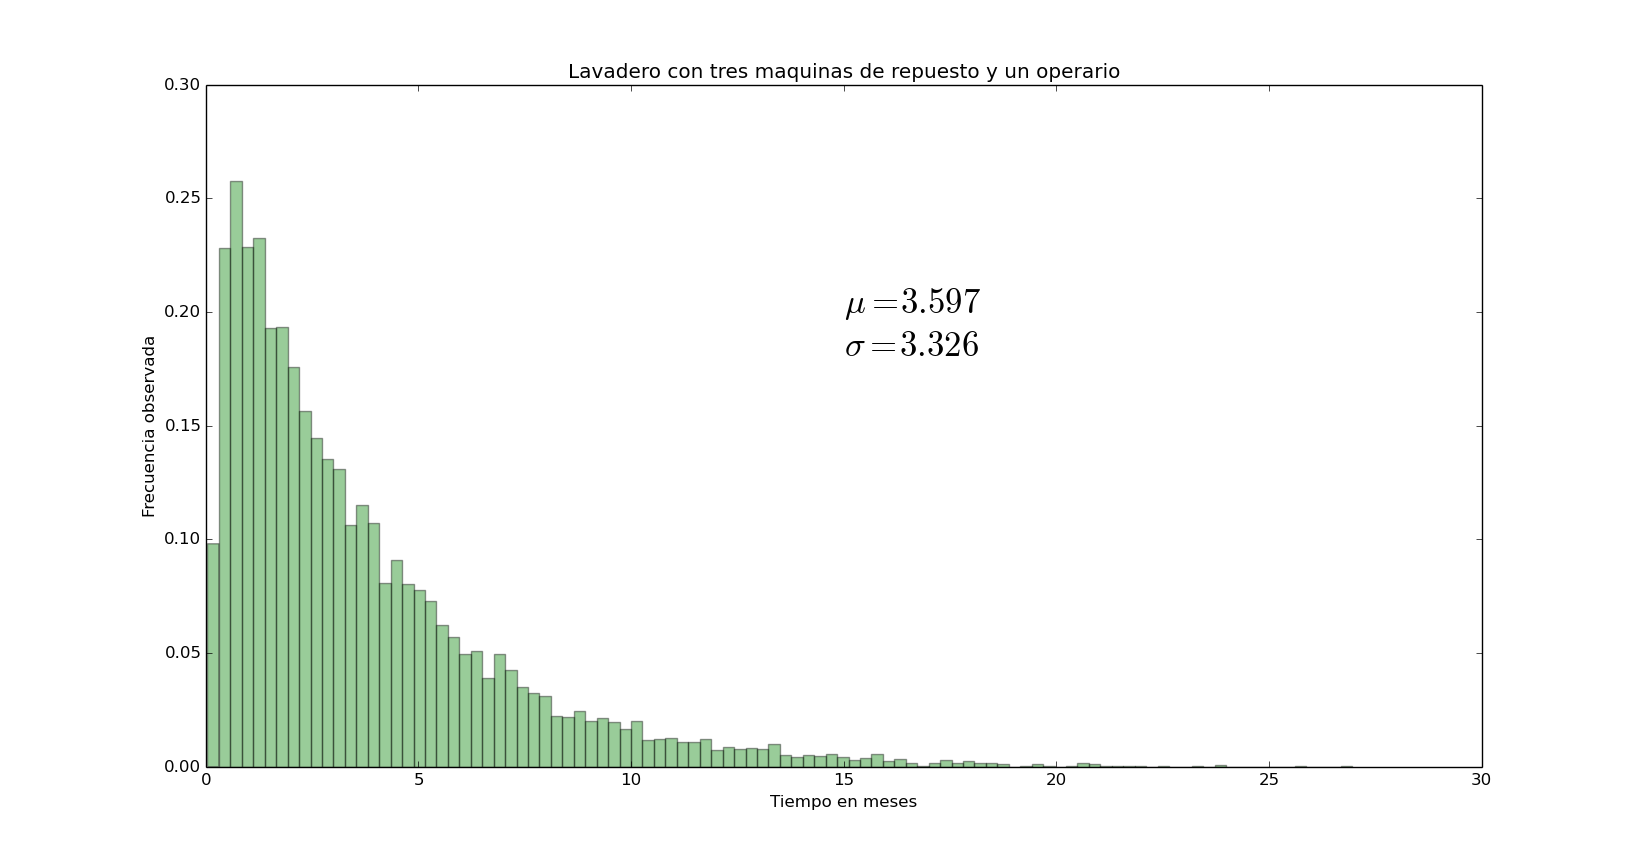
\includegraphics[scale=0.4]{figure_3}}
\end{figure}

Comparemos cómo ha cambiado el desempeño del sistema:

\begin{figure}[hbt]
\noindent\makebox[\textwidth]{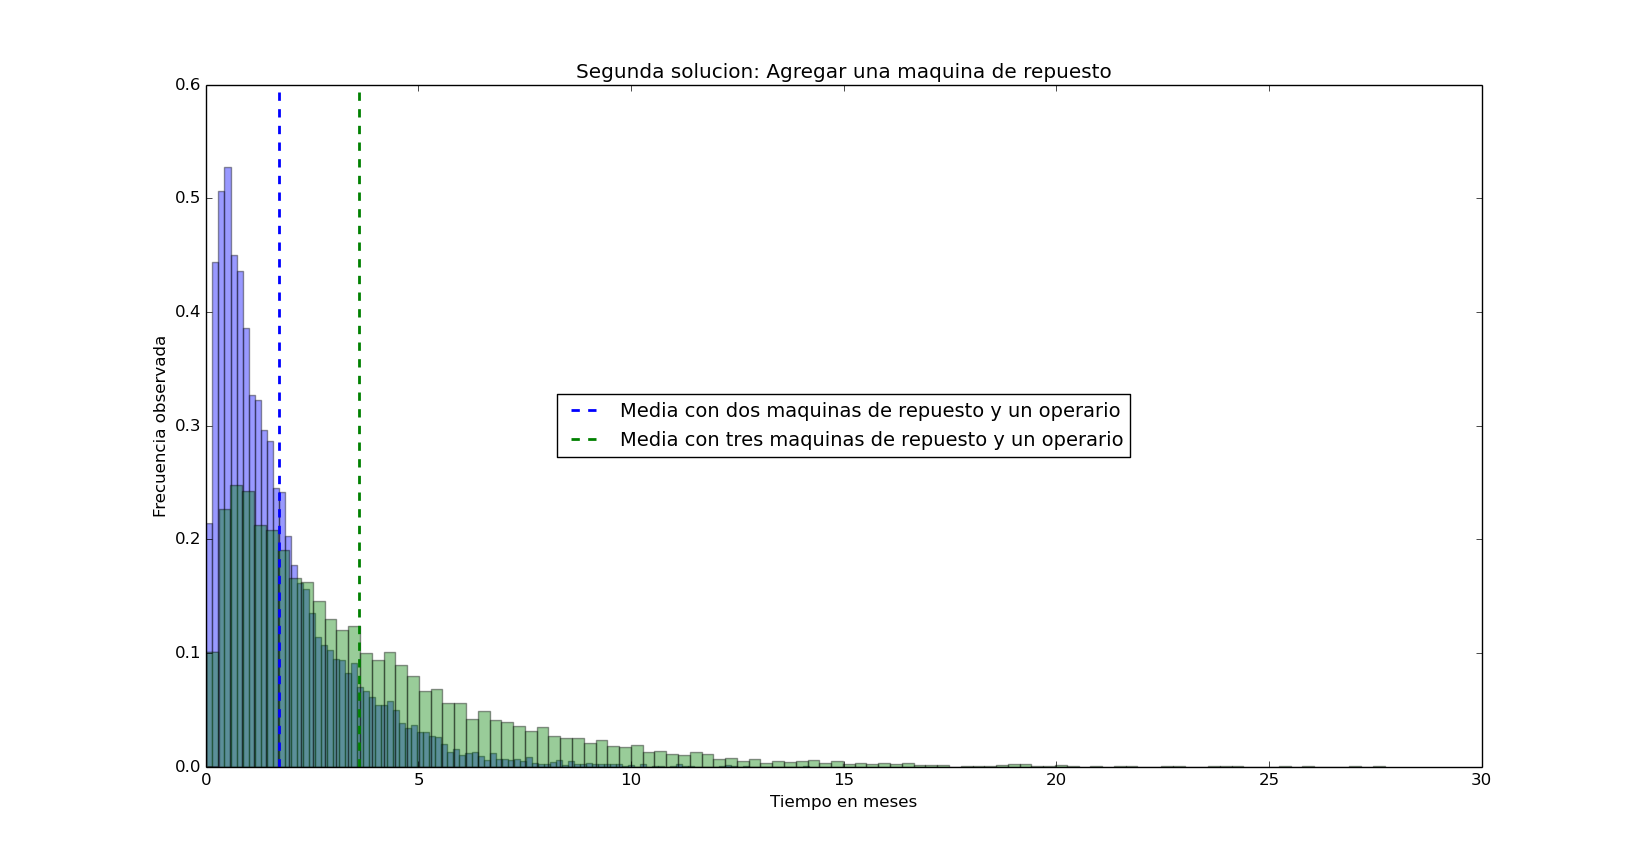
\includegraphics[scale=0.375]{figure_5}}
\end{figure}


\pagebreak

\subsection{Comparación entre las soluciones}

\begin{figure}[hbt]
\noindent\makebox[\textwidth]{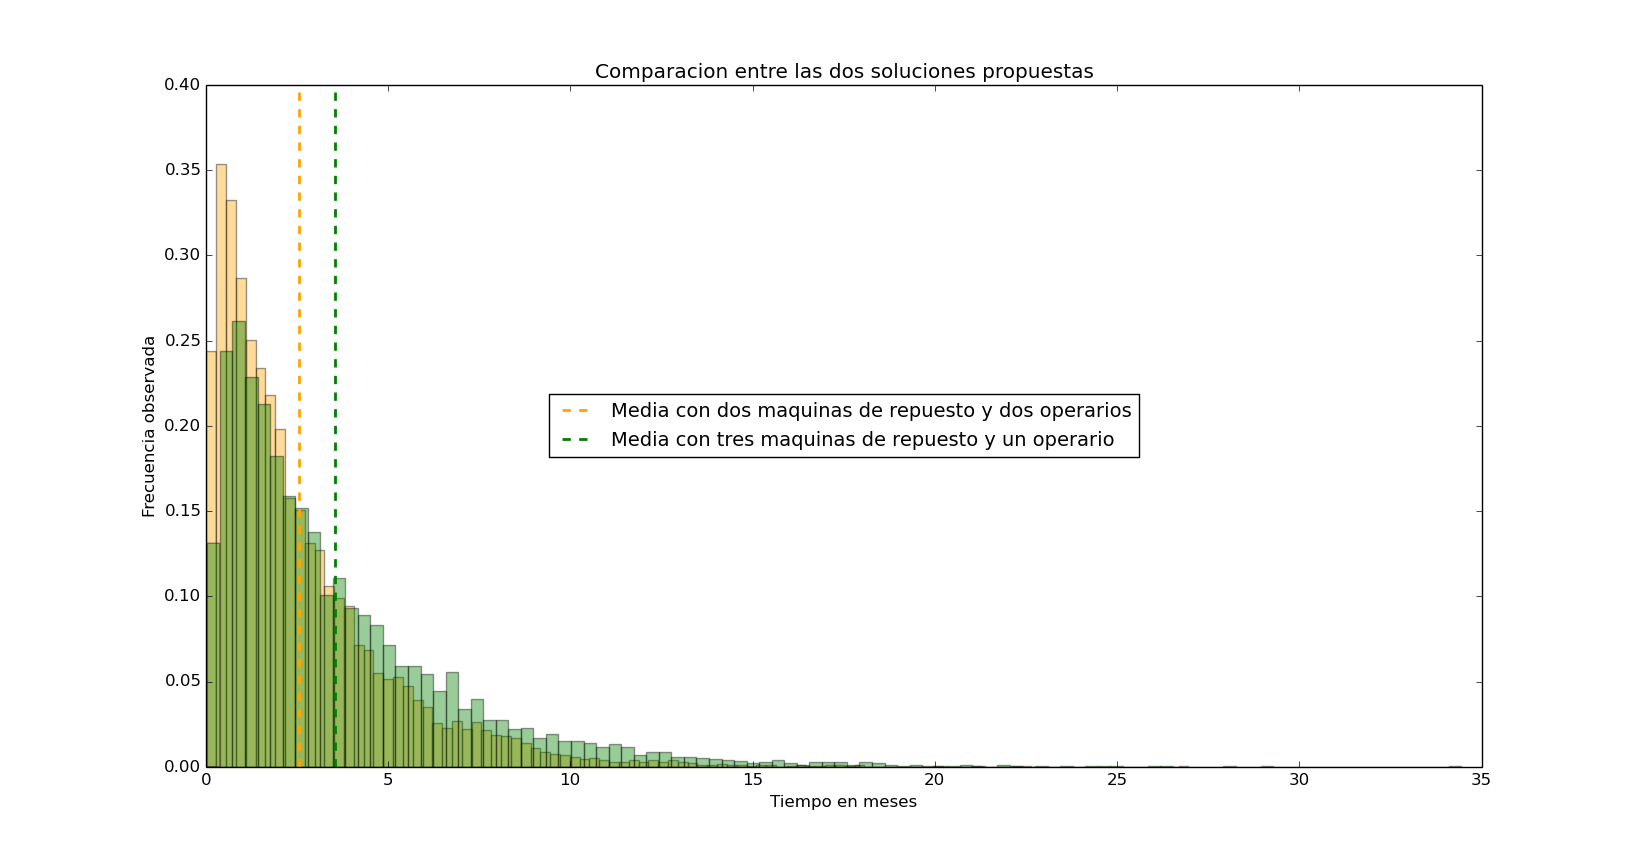
\includegraphics[scale=0.4]{figure_6}}
\end{figure}

Podemos notar que el sistema tiene mejor desempeño si agregamos una máquina en
vez de un operario.

\vspace{0.1in}
{\bf Comparación entre los tres sistemas:}


\begin{figure}[hbt]
\noindent\makebox[\textwidth]{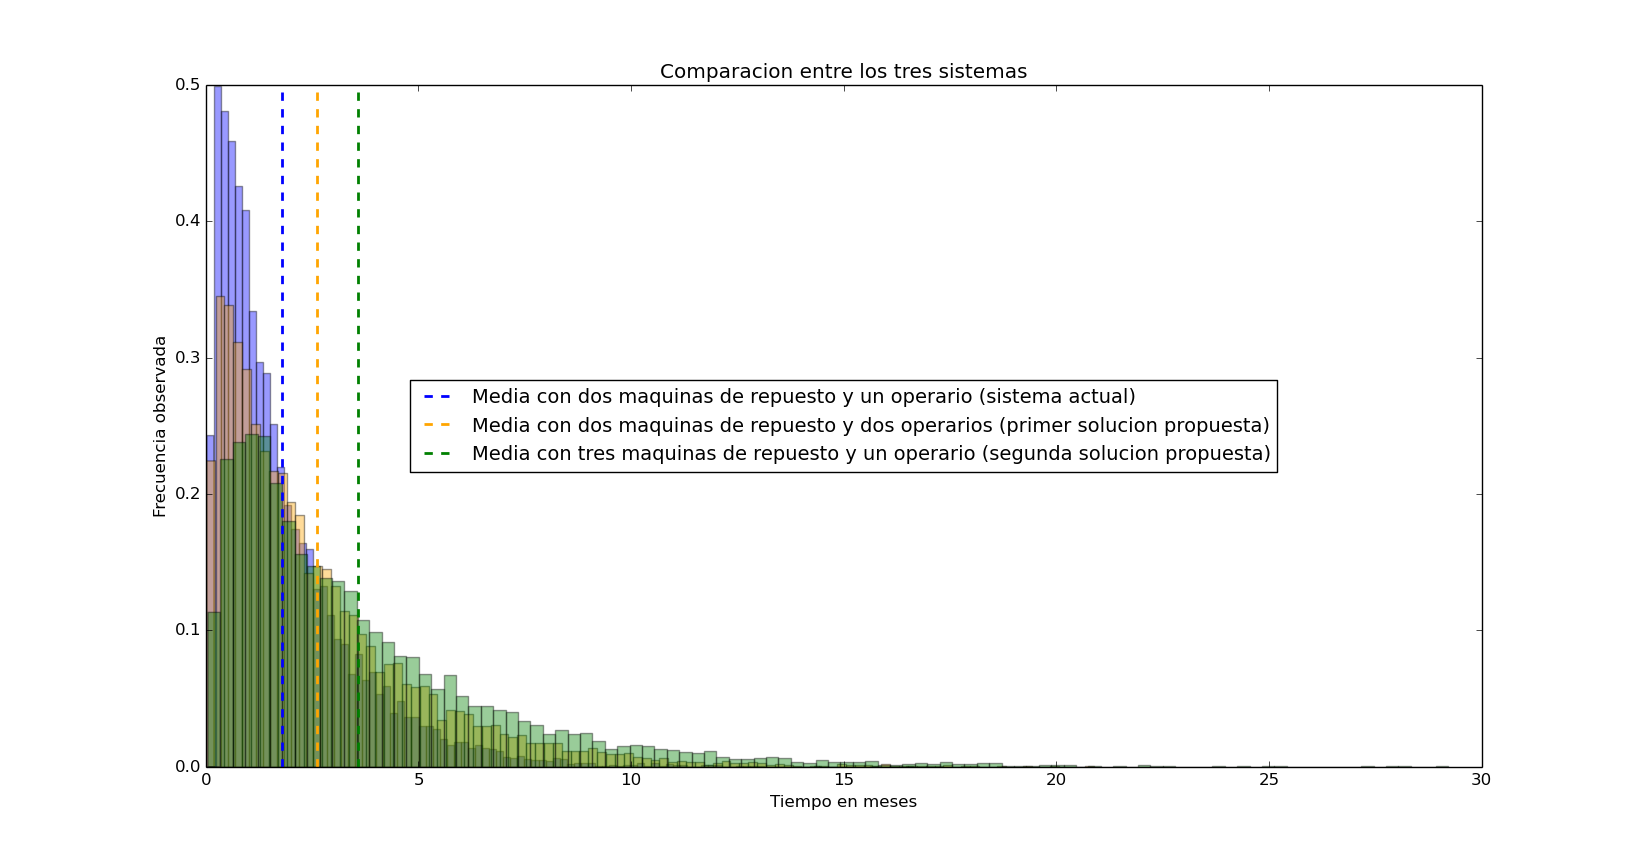
\includegraphics[scale=0.375]{figure_7}}
\end{figure}

\pagebreak

{\bf Tablas con las simulaciones}

\vspace{0.2in}
\begin{itemize}


\item\noindent{\bf 5 máquinas funcionando, 2 de repuesto y un operario}
\begin{center}
    \begin{tabular}{| l | l | l | l |}
    \hline
    N & $\mu$&$\sigma^2$&$\sigma$\\ \hline
    100 & 1.605& 2.573&1.545 \\ \hline
    1000 &1.761 &2.237 &1.652 \\ \hline
    10000 &1.772 &2.453 & 1.616 \\
    \hline
    \end{tabular}
\end{center}
\vspace{0.2in}
\item{\bf 5 máquinas funcionando, 2 de repuesto y dos operarios}
\begin{center}
    \begin{tabular}{| l | l | l | l |}
    \hline
    N & $\mu$&$\sigma^2$&$\sigma$\\ \hline
    100 & 2.651& 6.531&2.082 \\ \hline
    1000 &2.652 &5.689 &2.423 \\ \hline
    10000 &2.601 &6.445 & 2.438 \\
    \hline
    \end{tabular}
\end{center}
\vspace{0.2in}
\item{\bf 5 máquinas funcionando, 3 de repuesto y un operario}
\begin{center}
    \begin{tabular}{| l | l | l | l |}
    \hline
    N & $\mu$&$\sigma^2$&$\sigma$\\ \hline
    100 & 3.695& 11.799&2.899 \\ \hline
    1000 &3.517 &10.56 &3.397 \\ \hline
    10000 &3.628 &10.813 & 3.356 \\
    \hline
    \end{tabular}
\end{center}
\end{itemize}

\clearpage

\section{Conclusión}

Dados los resultados observados podemos ver que contando con ciertas bases teóricas y un poco de información
del problema que estamos modelando, podemos ser capaces de responder a incógnitas que parecen muy difíciles
de estimar. Incluso si supiéramos que un sistema con 5 máquinas funcionando, dos de repuesto y un operario,
tuviera una media de tiempo hasta que falla de 1.75 meses, no sería obvio saber si la media de tiempo hasta
que el sistema falla mejora agregando un operario o una máquina de repuesto.
Gracias a las hipótesis en las que nos basamos, fuimos capaces de observar, mediante simulaciones, que
la media de tiempo hasta que el sistema falla aumenta a 3.6 meses si ponemos una máquina más de repuesto;
contra 2.6 meses si agregamos un operario.

\end{document}